\documentclass[11pt,aspectratio=169]{beamer}
\usetheme{default}
\setbeamertemplate{navigation symbols}{}
\setbeamertemplate{footline}[frame number]
\setbeamercovered{invisible}
\usepackage{amsmath,amssymb}
\usepackage{booktabs}
\usepackage{pgfplots}
\pgfplotsset{compat=1.17}
\newcommand{\norm}[1]{\lVert #1\rVert}

\title{Tightening the error bound of the\\fourth-order Suzuki--Trotter formula}
\author{Areg Gevorgyan\\{\small University of Maryland, College Park \quad areg@umd.edu}}
\date{Caltech $\times$ SAIR Mathathon --- Problem \#109}

\begin{document}

\begin{frame}
\titlepage
\end{frame}

% ---------------------------------------------------------------
\begin{frame}{Simulating quantum dynamics with product formulas}
\begin{itemize}[<+->]
\item Goal: run $e^{-it(A+B)}$ on a quantum computer.
\item We can only apply $e^{-isA}$ and $e^{-isB}$ separately, so we alternate them in many short steps.
\item The fourth-order Suzuki formula $S_4$ is a standard, widely used choice.
\item More steps means more gates, so the error bound decides the cost of a simulation.
\end{itemize}
\end{frame}

% ---------------------------------------------------------------
\begin{frame}{The problem}
\begin{itemize}[<+->]
\item Standard rigorous bound (Childs, Su, Tran, Wiebe, Zhu, 2021):
 \[\norm{S_4(t)-e^{tH}}\ \le\ t^5\sum_w\gamma_w\norm{C_w},\qquad \textstyle\sum_w\gamma_w=0.0875,\]
 a weighted sum over 8 nested commutators $C_w$.
\item For fourth-order formulas this overestimates the true error by up to about three orders of magnitude.
\item Reason: the proof adds up absolute values of many terms that largely cancel.
\item Task: prove a rigorous bound with a strictly smaller prefactor, using the exact leading error term and a controlled remainder.
\end{itemize}
\end{frame}

% ---------------------------------------------------------------
\begin{frame}{Three sources of slack, three fixes}
\begin{enumerate}[<+->]
\item The leading $t^5$ term is bounded piece by piece.\\
 \quad $\Rightarrow$ compute it exactly.
\item The remainder is bounded before its terms can cancel.\\
 \quad $\Rightarrow$ reorganise the expansion so cancellations happen first.
\item The one-step bound is multiplied by the number of steps.\\
 \quad $\Rightarrow$ use the fact that part of the error cancels from step to step.
\end{enumerate}
\end{frame}

% ---------------------------------------------------------------
\begin{frame}{Fix 1: the exact leading error term}
\begin{itemize}[<+->]
\item $\log S_4(t)=tH+t^5E_5+\dots$, and $E_5$ is a combination of six nested commutators.
\item We found all six coefficients exactly, as numbers of the form $a+b\,2^{1/3}+c\,2^{2/3}$ with rational $a,b,c$.
\item Checked three ways: exact computer arithmetic, the Alkahest computer-algebra system, and a proof checked by the Lean theorem prover.
\item In the commutators Childs et al.\ use, the constants of $E_5$ sum to $0.0029982$, against their $0.0875$.
\end{itemize}
\end{frame}

% ---------------------------------------------------------------
\begin{frame}{Fix 2: a remainder that keeps cancellations}
\begin{itemize}[<+->]
\item Start from one Duhamel (variation-of-constants) identity, applied along the stages of the formula.
\item Expand so that every leftover exponential is a unitary rotation, which does not change norms.
\item Combine all terms that share a rotation into one exact expression before taking a norm.
\item Result: explicit, rigorous constants for the $t^6$ and $t^7$ corrections, valid for every step size.
\end{itemize}
\end{frame}

% ---------------------------------------------------------------
\begin{frame}{Single-step results}
\begin{center}
\begin{tabular}{@{}lll@{}}
\toprule
bound & form & constants\\
\midrule
Childs et al.\ 2021 & $t^5$ & $0.0875$\\
\pause Theorem A & $t^5$ & $0.01367$\\
\pause Theorem C & $t^5+t^6+t^7$ & $0.0029982+0.0004993+0.0006659$\\
\bottomrule
\end{tabular}
\end{center}
\begin{itemize}[<+->]
\item Theorem A: every coefficient is below the matching one of Childs et al., so it is better for every $H$.
\item Theorem C: the $t^5$ part is the exact leading term, $29\times$ smaller than Childs et al.
\end{itemize}
\end{frame}

% ---------------------------------------------------------------
\begin{frame}{Comparison on the Ising chain}
Ising chain with a transverse field, 8 spins; prefactors with this Hamiltonian's commutator norms:
\begin{center}
\begin{tabular}{@{}ll@{}}
\toprule
bound & prefactor\\
\midrule
Childs et al. & $94.17\,t^5$\\
Schubert--Mendl (2023), best split & $94.16\,t^5$\\
\pause Theorem A & $14.41\,t^5$\\
\pause Theorem C & $2.913\,t^5+1.466\,t^6+9.648\,t^7$\\
\pause exact leading term (not a bound) & $1.498\,t^5$\\
\bottomrule
\end{tabular}
\end{center}
\end{frame}

% ---------------------------------------------------------------
\begin{frame}{One step: bound divided by true error}
\centering
\begin{tikzpicture}
\begin{loglogaxis}[width=0.78\textwidth,height=0.62\textheight,xlabel={step size $t$},
 ylabel={bound / true error},legend pos=north west,legend style={font=\footnotesize},
 ymin=0.8,ymax=400]
\addplot[red,dashed,thick] coordinates {(0.005012,62.86) (0.006813,62.86) (0.009261,62.86) (0.01259,62.87) (0.01711,62.87) (0.02326,62.88) (0.03162,62.9) (0.04299,62.93) (0.05843,62.99) (0.07943,63.1) (0.108,63.31) (0.1468,63.69) (0.1995,64.39) (0.2712,65.69) (0.3687,68.14) (0.5012,72.79)};
\addlegendentry{Childs et al.}
\addplot[orange,thick] coordinates {(0.005012,9.617) (0.006813,9.617) (0.009261,9.617) (0.01259,9.618) (0.01711,9.618) (0.02326,9.62) (0.03162,9.622) (0.04299,9.627) (0.05843,9.637) (0.07943,9.654) (0.108,9.685) (0.1468,9.743) (0.1995,9.85) (0.2712,10.05) (0.3687,10.42) (0.5012,11.14)};
\addlegendentry{Theorem A}
\addplot[blue,thick] coordinates {(0.005012,1.95) (0.006813,1.951) (0.009261,1.954) (0.01259,1.958) (0.01711,1.963) (0.02326,1.971) (0.03162,1.983) (0.04299,2.001) (0.05843,2.028) (0.07943,2.071) (0.108,2.14) (0.1468,2.256) (0.1995,2.454) (0.2712,2.805) (0.3687,3.448) (0.5012,4.693)};
\addlegendentry{Theorem C}
\addplot[teal,dotted,very thick] coordinates {(0.005012,1.003) (0.006813,1.004) (0.009261,1.006) (0.01259,1.008) (0.01711,1.011) (0.02326,1.016) (0.03162,1.022) (0.04299,1.033) (0.05843,1.048) (0.07943,1.073) (0.108,1.113) (0.1468,1.18) (0.1995,1.294) (0.2712,1.496) (0.3687,1.866) (0.5012,2.582)};
\addlegendentry{our bound with this $H$'s norms}
\addplot[black,thin,domain=0.005:0.5] {1};
\end{loglogaxis}
\end{tikzpicture}

{\footnotesize Ising chain, 8 spins. Childs et al.\ is about $63\times$ the true error; Theorem C about $2\times$.}
\end{frame}

% ---------------------------------------------------------------
\begin{frame}{Fix 3: errors cancel across steps}
\begin{itemize}[<+->]
\item Part of the leading error has the form $[H,Y]$. Between steps it rotates and averages out instead of piling up.
\item This effect is known (Tran et al.\ 2020, Layden 2022, Y.-H.\ Chen 2025, B.\ Chen et al.\ 2026).
\item We make it fully explicit for $S_4$: only a remainder $Z$ accumulates, with constants $0.00089$ instead of $0.0030$.
\item Repeating the argument one order higher (Theorem D$'$) tightens the bound further for long simulations.
\end{itemize}
\end{frame}

% ---------------------------------------------------------------
\begin{frame}{Many steps: Trotter steps needed}
\centering
\begin{tikzpicture}
\begin{loglogaxis}[width=0.78\textwidth,height=0.62\textheight,xlabel={total time $T$},
 ylabel={steps for error $10^{-3}$},legend pos=north west,legend style={font=\footnotesize}]
\addplot[red,dashed,thick,mark=o] coordinates {(2,42) (8,236) (32,1334) (128,7543)};
\addlegendentry{Childs et al.}
\addplot[blue,thick,mark=square] coordinates {(2,15) (8,78) (32,426) (128,2380)};
\addlegendentry{Theorem D$'$, universal constants}
\addplot[teal,thick,mark=triangle] coordinates {(2,13) (8,62) (32,330) (128,1815)};
\addlegendentry{Theorem D$'$ with this $H$'s norms}
\addplot[black,very thick,mark=*] coordinates {(2,11) (8,56) (32,314) (128,1776)};
\addlegendentry{true}
\end{loglogaxis}
\end{tikzpicture}

{\footnotesize At $T=128$: $1815$ guaranteed vs.\ $1776$ needed ($+2.2\%$); Childs et al.\ $7543$.}
\end{frame}

% ---------------------------------------------------------------
\begin{frame}{How far from reality?}
Bound divided by true error at the step count that truly reaches error $10^{-3}$ (8 models, 8 qubits):
\begin{center}
\begin{tabular}{@{}lc@{}}
\toprule
& worst-case error\\
\midrule
Childs et al. & 320--740\\
\pause Theorem D$'$, universal constants & 3.1--10.7\\
\pause Theorem D$'$ with this $H$'s norms & 1.5--6.5\\
\bottomrule
\end{tabular}
\end{center}
\begin{itemize}[<+->]
\item Large Ising chains (exact, up to 1000 spins): our guaranteed step count is within $0.37\%$ of the true one at 1000 spins.
\end{itemize}
\end{frame}

% ---------------------------------------------------------------
\begin{frame}{The leading constant cannot be improved}
\begin{itemize}[<+->]
\item Question: could a different bound of the same commutator form have a smaller $t^5$ constant?
\item Each pair of test matrices gives a constraint any valid bound must satisfy.
\item Linear-programming duality turns six small matrix pairs into a lower bound: $0.0029981499$.
\item Our constant is $0.0029981584$, optimal to within 3 parts in a million.
\item The proof uses exact rational arithmetic.
\end{itemize}
\end{frame}

% ---------------------------------------------------------------
\begin{frame}{Machine-checked}
\begin{itemize}[<+->]
\item Lean 4 with Mathlib (v4.35.0), about 2100 lines, no unproved steps.
\item Formalised: the Duhamel identity, the remainder expansion for any product formula, and the many-step theorems.
\item Lean's kernel also checks the exact leading term.
\item Still outside Lean: the numerical values of the constants (computed in exact arithmetic in Python).
\end{itemize}
\end{frame}

% ---------------------------------------------------------------
\begin{frame}{Summary and next steps}
\begin{itemize}[<+->]
\item Exact leading error term of $S_4$ in closed form.
\item Rigorous bounds with prefactors $0.01367$ (single term) and $0.0029982$ (exact leading term) against $0.0875$.
\item Many-step guarantees within a few percent of the true step count.
\item The leading constant is provably optimal; the analysis is machine-checked.
\item Next: connect the numerical constants to Lean, extend to more than two terms and to other formulas.
\end{itemize}
\vspace{0.8em}
\end{frame}

\end{document}
